\chapter{Kleinste Zahl in einem Array finden}

\TopicLevel{Arrays}{1}

\begin{enumerate}
  \item Erstellen Sie ein Programm, welches aus einem gegebenen Array aus
  Zahlen die kleinste Zahl ermittelt.

\Vorlage
\begin{minted}{c}
#include <stdio.h>

int main(void) {
    int myArray[] = {4, 2, 9, 24, 4, 8, 5, 24};

    int min;
    // Durchsuchen Sie das Array nach dem kleinsten
    // Element ...

    printf("Kleinstes Element: %d\n", min);
}
\end{minted}

\begin{mybox}[Bildschirmausgabe]{console}
Kleinstes Element: 2
\end{mybox}

\item Verändern Sie Ihr Programm derart, dass es eine eigene Funktion
\mintinline{c}{find_min()} gibt, die als Argumente ein Array aus Zahlen und die
Größe des Arrays entgegennimmt, und den kleinsten Wert aus dem Array an den
Aufrufer zurückliefert.
\end{enumerate}




\chapter{Häufigkeiten eines Werts in einem Array zählen}

\TopicLevel{Arrays}{1}

\begin{enumerate}
  \item Erstellen Sie ein Programm, welches aus einem gegebenen Array aus
  Ganzzahlen und einer vorgegebenen Zahl die Häufigkeit ausgibt, mit der diese
  Zahl im Array vorkam.

\Vorlage
\begin{minted}{c}
#include <stdio.h>

int main(void) {
    int myArray[] = {4, 2, 9, 24, 4, 8, 5, 24};
    int to_find = 4;

    int count;
    // Zählen Sie, wie häufig die Zahl to_find
    // im Array vorkommt ...

    printf("Anzahl in Array: %d\n", count);
}
\end{minted}

\begin{mybox}[Bildschirmausgabe]{console}
Anzahl in Array: 2
\end{mybox}

  \item Verändern Sie Ihr Programm derart, dass es eine eigene Funktion
  \mintinline{c}{occurrences()} gibt, die diese Operation durchführt und die
  Häufigkeit der gesuchten Zahl an den Aufrufer zurückliefert.

  Überlegen Sie sich, welche Parameter eine solche Funktion benötigt.

\end{enumerate}



\chapter{Reihenfolge eines Arrays umkehren}

\TopicLevel{Arrays}{1}

\begin{enumerate}
    \item Erstellen Sie ein Programm, welches die Reihenfolge eines gegebenen
    Arrays aus Zahlen umkehrt.

\Vorlage
\begin{minted}{c}
#include <stdio.h>

int main(void) {
    int myArray[] = {4, 2, 9, 24, 4, 8, 5, 24};

    // Kehren Sie die Reihenfolge der Zahlen des
    // Arrays um ...

    printf("Umgekehrte Reihenfolge:\n");

    // Geben Sie die umgekehrte Reihenfolge aus ...
}
\end{minted}

\begin{mybox}[Bildschirmausgabe]{console}
Umgekehrte Reihenfolge:
myArray[0] = 24
myArray[1] = 5
myArray[2] = 8
myArray[3] = 4
myArray[4] = 24
myArray[5] = 9
myArray[6] = 2
myArray[7] = 4
\end{mybox}

  \item Verändern Sie Ihr Programm derart, dass es eine eigene Funktion
  \mintinline{c}{reverse()} gibt, die als Argumente ein Array aus Zahlen und die
  Größe des Arrays entgegennimmt, und die Reihenfolge der Zahlen im übergebenen
  Array umkehrt.
\end{enumerate}



\chapter{Länge des kürzesten Wortes in einem Satz bestimmen}

\TopicLevel{Arrays und Strings}{1}\vspace{10pt}

Erstellen Sie eine Funktion \mintinline{c}{shortestWordLength()}, die die Länge
des kürzesten Wortes in einem gegebenen Satz ermittelt. Der Funktion wird eine
Zeichenkette übergeben, die aus Wörtern besteht, die durch Leerzeichen getrennt
sind. Die Funktion soll die Länge des kürzesten Wortes berechnen und diesen Wert
an den Aufrufer zurückgeben.

\Vorlage
\begin{minted}{c}
int main(void) {
    char string1[] = "Ein Tag am Meer";
    printf("\"%s\"\n", string1);
    printf("Kürzestes Wort hat %d Zeichen\n", shortestWordLength(string1));

    char string2[] = "Fischers Fritze fischt frische Fische";
    printf("\"%s\"\n", string2);
    printf("Kürzestes Wort hat %d Zeichen\n\n", shortestWordLength(string2));
}
\end{minted}

\begin{mybox}[Bildschirmausgabe]{console}
"Ein Tag am Meer"
Kürzestes Wort hat 2 Zeichen

"Fischers Fritze fischt frische Fische"
Kürzestes Wort hat 6 Zeichen
\end{mybox}




\chapter{Text in Leetspeak umwandeln}

\TopicLevel{Strings}{1}\vspace{10pt}

Im sog. \textit{Leetspeak} werden bestimmte Buchstaben durch ähnlich aussehende
Zeichen oder Ziffern ersetzt. Beispielsweise würde "\textsf{1337 5P34K}" dem
Wort "\textsf{Leet Speak}" entsprechen.

\begin{enumerate}
\item Erstellen Sie eine Funktion \mintinline{c}{getLeetChar()}, die ein Zeichen
als Argument erhält, dieses nach den Leetspeak-Regeln ersetzt (falls zutreffend)
und das konvertierte oder unveränderte Zeichen zurückgibt. Die Ersetzung erfolgt
sowohl für Groß- als auch für Kleinbuchstaben nach folgendem Schema:

\texttt{A} $\rightarrow$ \texttt{4} \tab \texttt{B} $\rightarrow$ \texttt{8} \tab \texttt{E} $\rightarrow$ \texttt{3} \tab \texttt{G} $\rightarrow$ \texttt{6}

\texttt{H} $\rightarrow$ \texttt{\#} \tab \texttt{I} $\rightarrow$ \texttt{1} \tab \texttt{O} $\rightarrow$ \texttt{0} \tab \texttt{S} $\rightarrow$ \texttt{\$}

\texttt{T} $\rightarrow$ \texttt{7} \tab \texttt{Z} $\rightarrow$ \texttt{2}

\item Erstellen Sie anschließend eine Funktion \mintinline{c}{leetspeak()}, die
einen String als Argument entgegennimmt und mithilfe der Funktion
\mintinline{c}{getLeetChar()} jedes Zeichen des übergebenen Strings prüft und
ggf. verändert. Der gesamte String soll schließlich von der Funktion in
Leetspeak umgewandelt werden.

\Vorlage
\begin{minted}[fontsize=\small]{c}
#include <stdio.h>

int main(void) {
    char input[100];

    printf("Satz eingeben: ");
    fgets(input, sizeof(input), stdin);

    // Folgende Funktion sollen Sie erstellen:
    leetspeak(input);

    printf("Leetspeak: %s", input);

    return 0;
}
\end{minted}

\begin{mybox}[Bildschirmausgabe]{console}
Satz eingeben: \highlight{Das ist ein Test}
Leetspeak: D4$ 1$7 31n 73$7

Satz eingeben: \highlight{Hallo Welt}
Leetspeak: #4ll0 W3l7

Satz eingeben: \highlight{C-Programmierung macht Spaß}
Leetspeak: C-Pr06r4mm13run6 m4c#7 $p4ß
\end{mybox}
\end{enumerate}



\chapter{Barcode-Prüfziffer berechnen}

\TopicLevel{Arrays und Strings}{2}\vspace{10pt}

In der folgenden Aufgabe geht es darum, die Prüfziffer eines EAN-Barcodes zu
berechnen. Ein EAN-Barcode besteht aus insgesamt 13 Ziffern, wovon die letzte
Ziffer die Prüfziffer ist.

\begin{figure}[htb!]
\centering
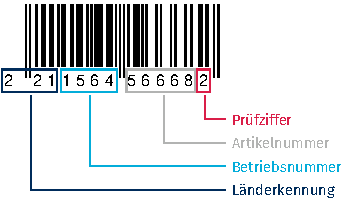
\includegraphics[width=.6\textwidth]{barcode}
\end{figure}

\begin{enumerate}

\item Erstellen Sie eine Funktion \mintinline{c}{convertStringToArray()}, die
aus einem String ein Array aus Ganzzahlen erzeugt. Die Funktion bekommt sowohl
den String als auch das Array als Funktionsargumente übergeben.

Führen Sie in der Funktion Überprüfungen durch, ob die Länge des Strings die
Größe \mintinline{c}{BARCODE_LENGTH} nicht überschreitet und ob es sich bei
jedem Zeichen um eine Zahl handelt (verwenden Sie hierfür die
\mintinline{c}{isdigit()}-Funktion der Standardbibliothek). Schlägt eine der
beiden Überprüfungen fehl, so soll die Funktion
\mintinline{c}{convertStringToArray} eine Fehlermeldung aus- und einen Wert
ungleich 0 zurückgeben. Andernfalls gibt sie den Wert 0 zurück.

\textit{Hinweis:} Zeichen werden in C durch \textit{ASCII-Werte} dargestellt.
Der ASCII-Wert des Zeichens \texttt{'0'} ist beispielsweise 48. Um eine
Zeichenziffer (z.\,B. \texttt{'5'}) in ihre entsprechende numerische Ziffer
(z.\,B. 5) zu konvertieren, müssen Sie den ASCII-Wert des Zeichens \texttt{'0'}
von dem aktuellen Zeichen subtrahieren.

\pagebreak

\Vorlage
\begin{minted}[fontsize=\small]{c}
#include <stdio.h>
#include <string.h> // für strlen() und strcspn()
#include <ctype.h>  // für isdigit()

#define BARCODE_LENGTH 12

int main(void) {
    // Eingabe String: Platz für 12 Ziffern + Nullterminator
    char inputString[BARCODE_LENGTH + 1];
    int barcode[BARCODE_LENGTH];

    printf("Ersten 12 Ziffern des EAN-13 Barcodes eingeben:\n");
    fgets(inputString, sizeof(inputString), stdin);

    // Entfernt das Newline-Zeichen, falls vorhanden,
    // und ersetzt es durch das Nullterminierungszeichen
    inputString[strcspn(inputString, "\n")] = 0;


    // (a) Die Funktion convertStringToArray müssen Sie
    //     implementieren
    int convertResult = convertStringToArray(inputString, barcode);

    if (convertResult != 0)
        return 1; // String konnte nicht konvertiert werden

    // Testen der Funktion
    for (int i = 0; i < BARCODE_LENGTH; i++)
        printf("%d ", barcode[i]);
    printf("\n");

    return 0;
}
\end{minted}

\begin{mybox}[Bildschirmausgabe]{console}
Ersten 12 Ziffern des EAN-13 Barcodes eingeben:
\highlight{459876342178}
4 5 9 8 7 6 3 4 2 1 7 8
\end{mybox}



\pagebreak

\item Erstellen Sie eine Funktion \mintinline{c}{barcodeCheckDigit()}, die die
Prüfziffer eines EAN-13 Barcodes berechnet. Die Funktion bekommt die Ziffern in
Form eines Integer-Arrays, sowie die Länge des Arrays als Funktionsargumente
übergeben und berechnet die Prüfziffer nach dem folgenden Algorithmus:

\begin{enumerate}[1.]
    \item Addieren Sie die Ziffern an den ungeraden Positionen (Ziffern 1, 3, 5,
    etc.)
    \item Addieren Sie die Ziffern an den geraden Positionen (Ziffern 2, 4, 6,
    etc.) und multiplizieren Sie das Ergebnis anschließend mit 3
    \item Addieren Sie die beiden Ergebnisse zusammen
    \item Berechnen Sie den Wert der Gesamtsumme modulo 10 (also den Rest bei
    der Division durch 10)
    \item Subtrahieren Sie das Ergebnis von 10, um die Prüfziffer zu ermitteln
    (falls das Ergebnis 10 ist, setzen Sie die Prüfziffer auf 0)
\end{enumerate}

\Vorlage
\begin{minted}[fontsize=\small]{c}
#include <stdio.h>
#include <string.h> // für strlen() und strcspn()
#include <ctype.h>  // für isdigit()

#define BARCODE_LENGTH 12

int main(void) {
    // Eingabe String: Platz für 12 Ziffern + Nullterminator
    char inputString[BARCODE_LENGTH + 1];
    int barcode[BARCODE_LENGTH];

    printf("Ersten 12 Ziffern des EAN-13 Barcodes eingeben:\n");
    fgets(inputString, sizeof(inputString), stdin);

    // Entfernt das Newline-Zeichen, falls vorhanden,
    // und ersetzt es durch das Nullterminierungszeichen
    inputString[strcspn(inputString, "\n")] = 0;


    // (a) String in Integer-Array umwandeln
    int convertResult = convertStringToArray(inputString, barcode);

    if (convertResult != 0)
        return 1; // String konnte nicht konvertiert werden

    // (b) Die Funktion barcodeCheckDigit müssen Sie
    //     implementieren
    int checkDigit = barcodeCheckDigit(barcode, BARCODE_LENGTH);

    // Ausgabe der Prüfziffer
    printf("Die Prüfziffer lautet: %d\n", checkDigit);

    return 0;
}
\end{minted}

\begin{mybox}[Bildschirmausgabe]{console}
Ersten 12 Ziffern des EAN-13 Barcodes eingeben:
\highlight{459876342178}
Die Prüfziffer lautet: 2

Ersten 12 Ziffern des EAN-13 Barcodes eingeben:
\highlight{0799439112766}
Die Prüfziffer lautet: 6

Ersten 12 Ziffern des EAN-13 Barcodes eingeben:
\highlight{460566400005}
Die Prüfziffer lautet: 0
\end{mybox}

\end{enumerate}



\chapter{Überprüfen, ob ein String ein Palindrom ist}

\TopicLevel{Strings}{2}\vspace{10pt}

Ein Palindrom ist ein Wort, eine Phrase, eine Zahl oder eine andere Sequenz von
Zeichen, die vorwärts und rückwärts gelesen identisch ist. Typische Beispiele
für Palindrome sind Wörter wie "Anna" oder "Otto", bei denen die Buchstabenfolge
von beiden Enden aus gleich bleibt.

Erstellen Sie eine Funktion \mintinline{c}{isPalindrome()}, die überprüft, ob
eine gegebene Zeichenkette (String) ein Palindrom ist. Die Funktion soll
\mintinline{c}{true} zurückgeben, wenn der String ein Palindrom ist, und
\mintinline{c}{false}, wenn er keines ist. Berücksichtigen Sie dabei, dass bei
der Überprüfung Groß- und Kleinschreibung ignoriert werden sollte.

\Vorlage
\begin{minted}{c}
#include <stdio.h>
#include <stdbool.h>

int main(void) {
    char string1[] = "Kein Palindrom";
    char string2[] = "Reliefpfeiler";   // ist ein Palindrom
    char string3[] = "Rentner";         // ist ein Palindrom

    // Die im Folgenden genutzte isPalindrome()-Funktion
    // müssen Sie erstellen

    if (isPalindrome(string1))
        printf("\"%s\" ist ein Palindrom\n", string1);
    else
        printf("\"%s\" ist kein Palindrom\n", string1);

    if (isPalindrome(string2))
        printf("\"%s\" ist ein Palindrom\n", string2);
    else
        printf("\"%s\" ist kein Palindrom\n", string2);

    if (isPalindrome(string3))
        printf("\"%s\" ist ein Palindrom\n", string3);
    else
        printf("\"%s\" ist kein Palindrom\n", string3);
}
\end{minted}

\begin{mybox}[Bildschirmausgabe]{console}
"Kein Palindrom" ist kein Palindrom
"Reliefpfeiler" ist ein Palindrom
"Rentner" ist ein Palindrom
\end{mybox}




\chapter{Strings unter Verwendung dynamischer Speicherzuweisung verbinden}

\TopicLevel{Strings, Dynamische Speicherverwaltung}{2}\vspace{10pt}

Erstellen Sie eine Funktion \mintinline{c}{stringAppend()}, die zwei Strings als
Eingabeparameter entgegennimmt und diese miteinander verbindet. Die Funktion
soll für den neuen, verbundenen String dynamisch Speicher auf dem Heap
reservieren und einen Pointer auf diesen Speicher an den Aufrufer zurückgeben.

\Vorlage
\begin{minted}{c}
#include <stdio.h>
#include <string.h>
#include <stdlib.h>

int main(void) {
    char first[] = "Übungsaufgaben Programmieren ";
    char second[] = "in C";

    char *newString = stringAppend(first, second);
    printf("%s\n", newString);

    free(newString);
}
\end{minted}

\begin{mybox}[Bildschirmausgabe]{console}
Übungsaufgaben Programmieren in C
\end{mybox}





\chapter{Häufigste vorkommende Zeichen in einem String finden}

\TopicLevel{Strings}{2}\vspace{10pt}

Erstellen Sie eine Funktion \mintinline{c}{printMaxChars()}, die basierend auf
einem an die Funktion übergebenen String das Zeichen ermittelt, das am
häufigsten in diesem String vorkommt und sowohl das Zeichen als auch die Anzahl
auf dem Bildschirm ausgibt.

\Vorlage
\begin{minted}{c}
#include <stdio.h>
#include <string.h>

int main(void) {
    char string[] = "Fischers Fritze fischt frische Fische, frische Fische fischt Fischers Fritze";

    printMaxChars(string);
}
\end{minted}

\begin{mybox}[Bildschirmausgabe]{console}
Zeichen i kommt 10 mal vor.
\end{mybox}





\chapter{Quadratzahlen der Ziffern einer Zahl zusammensetzen}

\TopicLevel{Zahlen}{2}\vspace{10pt}

Erstellen Sie eine Funktion \mintinline{c}{digitsToSquares()}, die für jede
Ziffer einer gegebenen Zahl \mintinline{c}{number} das Quadrat der Ziffer
berechnet und die Quadrate in der ursprünglichen Reihenfolge der Ziffern
zusammensetzt. Die Funktion soll eine Zahl zurückgeben, die die berechneten
Quadrate aller Ziffern von \mintinline{c}{number} enthält.

\Vorlage
\begin{minted}{c}
#include <stdio.h>

int main(void) {
    unsigned int inputNumber1 = 123;
    unsigned long long outputNumber1 = digitsToSquares(inputNumber1);
    printf("%u --> %lld\n", inputNumber1, outputNumber1);

    unsigned int inputNumber2 = 9119;
    unsigned long long outputNumber2 = digitsToSquares(inputNumber2);
    printf("%u --> %lld\n", inputNumber2, outputNumber2);

    unsigned int inputNumber3 = 3210987654;
    unsigned long long outputNumber3 = digitsToSquares(inputNumber3);
    printf("%u --> %lld\n", inputNumber3, outputNumber3);
}
\end{minted}

\begin{mybox}[title=Bildschirmausgabe]{console}
123 --> 149
9119 --> 811181
3210987654 --> 9410816449362516
\end{mybox}




\chapter{Anzahl Wörter in einem String zählen}

\TopicLevel{Strings}{3}\vspace{10pt}

Erstellen Sie eine Funktion \mintinline{c}{countWords()}, die zählt, wie häufig
ein Wort innerhalb einer Zeichenkette (String) vorkommt. Die Funktion soll das
Wort und die Zeichenkette als Eingabeparameter entgegennehmen und die Anzahl an
den Aufrufer zurückliefern. Berücksichtigen Sie dabei, dass bei der Überprüfung
Groß- und Kleinschreibung ignoriert werden sollen.

\Vorlage
\begin{minted}{c}
#include <stdio.h>

int main(void) {
    char string[] = "Fischers Fritze fischt frische Fische, frische Fische fischt Fischers Fritze";
    char word[] = "Fische";

    // Die im Folgenden genutzte countWords()-Funktion
    // müssen Sie erstellen
    int count = countWords(string, word);

    printf("Das Wort \"%s\" kam %d-mal im String vor", word, count);
}
\end{minted}

\begin{mybox}[Bildschirmausgabe]{console}
Das Wort "Fische" kam 2-mal im String vor
\end{mybox}



\chapter{Durchschnitt von Gruppen von Zahlen in einer Datei finden}

\TopicLevel{Dateioperationen}{3}\vspace{10pt}

Erstellen Sie ein Programm, das aus einer Textdatei eine Zeile einliest, in der
Zahlen in spezieller Gruppierung vorliegen. Die Anzahl der Zahlen einer jeden
Gruppe wird durch die erste Zahl der Gruppe angegeben.

Bei einer Datei mit folgendem Inhalt:

\begin{mybox}[Textdatei.txt]{file}
\highlight{5} 24 13 83 22 4 \highlight{3} 99 23 45 \highlight{4} 82 34 11 9 \highlight{6} 13 22 93 42 85 34
\end{mybox}

Gibt die erste Zahl \mintinline{text}{5} an, dass die nächsten fünf Zahlen zu
einer Gruppe gehören. Die nach dieser Gruppe stehende Zahl \mintinline{text}{3}
gibt dann an, dass die nächsten drei Zahlen zur nächsten Gruppe gehören, und so
weiter.

Das Programm soll nun für jede Gruppe alle zugehörigen Zahlen einlesen und den
Durchschnitt der Zahlen ermitteln. Z.B. soll die Ausgabe für die obenstehenden
Zahlen folgendes ergeben:

\begin{mybox}[Bildschirmausgabe]{console}
Gruppe mit 5 Elementen: 29.20
Gruppe mit 3 Elementen: 55.67
Gruppe mit 4 Elementen: 34.00
Gruppe mit 6 Elementen: 48.17
\end{mybox}




\chapter{Jüngste Person in einer Datenstruktur finden}

\TopicLevel{Strukturen, Pointer}{3}\vspace{10pt}

Erstellen Sie eine Funktion, welche aus einem Array an Personen nach der
jüngsten Person sucht. Die Funktion soll einen Pointer auf ein Array übergeben
bekommen, welches seinerseits Pointer auf Strukturen von Personen enthält. Jede
Person-Struktur enthält einen Vornamen, einen Nachnamen und ein Alter.

Die Funktion soll nun die Einträge des Arrays nach der jüngsten Person
durchsuchen und einen Pointer auf diesen Array-Eintrag zurückliefern.

\Vorlage
\begin{minted}{c}
#include <stdio.h>

typedef struct {
    char firstName[50];
    char lastName[50];
    int age;
} Person;

int main(void) {
    Person person1 = {"Max", "Mustermann", 30};
    Person person2 = {"Anna", "Schmidt", 25};
    Person person3 = {"John", "Doe", 40};

    Person *persons[] = {&person1, &person2, &person3};

    int size = sizeof(persons) / sizeof(persons[0]);

    Person *youngest = findYoungestPerson(persons, size);

    printf("Name: %s %s, Age: %d\n", youngest->firstName, youngest->lastName, youngest->age);

    return 0;
}
\end{minted}

\begin{mybox}[Bildschirmausgabe]{console}
Name: Anna Schmidt, Age: 25
\end{mybox}


Man kann sich die Struktur also wie folgt vorstellen:

\begin{figure}[htb!]
\begin{tikzpicture}[font=\ttfamily]
    % Definiere Stil für die Array-Boxen
    \tikzstyle{array} = [rectangle, draw, minimum width=1cm, minimum height=1cm, anchor=north]

    % Definiere Stil für die Pointer
    \tikzstyle{pointer} = [circle, fill, inner sep=2pt]

    % Definiere Stil für die Struktur-Boxen
    \tikzstyle{struct} = [rectangle split, rectangle split parts=3, draw, text centered, minimum width=3cm, anchor=west]

    % Definiere Stil für die Pfeile
    \tikzstyle{arrow} = [-{Latex[length=3mm, width=2mm]}]

    % Erste Array-Box, Pointer und Struktur
    \node[array] (array0) at (0,0) {};
    \node[pointer] (pointer0) at (array0.center) {};
    \node[struct] (struct0) at (2, 0) {Max\nodepart{second}Mustermann\nodepart{third}30};

    % Zweite Array-Box, Pointer und Struktur
    \node[array] (array1) [below=0cm of array0] {};
    \node[pointer] (pointer1) at (array1.center) {};
    \node[struct] (struct1) at (2, -2) {Anna\nodepart{second}Schmidt\nodepart{third}25};

    % Dritte Array-Box, Pointer und Struktur
    \node[array] (array2) [below=0cm of array1] {};
    \node[pointer] (pointer2) at (array2.center) {};
    \node[struct] (struct2) at (2, -4) {John\nodepart{second}Doe\nodepart{third}40};

    % Zeichne Pfeile von Pointern zu Strukturen
    \foreach \x in {0,1,2}
        \draw[arrow] (pointer\x) -- (struct\x.text west);

    % Beschriftung der Array-Elemente
    \foreach \x in {0,1,2}
        \node at (array\x.west) [left] {persons[\x]};
\end{tikzpicture}
\end{figure}




\chapter{Verkettete Liste erstellen}

\TopicLevel{Strukturen, Pointer}{5}\vspace{10pt}

Erstellen Sie eine Datenstruktur in Form einer verketteten Liste, die es Ihnen
erlaubt, dynamisch eine beliebige Anzahl an Elementen zu Ihrer Liste
hinzuzufügen oder daraus zu entfernen.

Eine verkettete Liste besteht aus einer Menge an Knoten, die jeweils Daten
enthalten, sowie einen Pointer auf den nächsten Knoten in der Liste. Im letzten
Knoten der Liste enthält der Pointer auf den nächsten Knoten den Wert
\mintinline{c}{NULL}. Daran kann man erkennen, dass man am Ende der Liste
angekommen ist.

Die Knoten einer verketteten Liste können prinzipiell beliebige (aber
gleichartige) Daten enthalten. In unserem Beispiel reicht es uns, wenn einfach
ein Integer-Wert pro Knoten gespeichert wird.

Eine Liste mit drei Knoten und den Daten \mintinline{c}{4}, \mintinline{c}{2}
und \mintinline{c}{7} können Sie sich wie folgt vorstellen:

\begin{figure}[htb!]
    \begin{tikzpicture}[font=\ttfamily, node distance=1.2cm]
        % Definiere Stil für die Struktur-Boxen
        \tikzstyle{struct} = [
            rectangle split,    % Rechteck, das in mehrere Teile unterteilt ist
            rectangle split parts=2, % Rechteck besteht aus zwei Teilen
            draw,               % Umriss des Knotens zeichnen
            text centered,
            minimum width=1.5cm,
            anchor=base         % Positionierung relativ zu anderen Objekten auf die
                                % Basislinie des Textes im Knoten
        ]

        % Definiere Stil für die Liste-Box
        \tikzstyle{liststruct} = [
            rectangle,
            draw,
            text centered,
            minimum width=1.5cm
        ]

        % Definiere Stil für die Pointer
        \tikzstyle{pointer} = [circle, fill, inner sep=2pt]

        % Definiere Stil für die Pfeile
        \tikzstyle{arrow} = [-{Latex[length=3mm, width=2mm]}]

        % Listenstruktur
        \node[liststruct] (list) {head};
        \node[above=0 of list, font=\sffamily] {Liste};
        \node[pointer] (pointerList) at ([xshift=-6pt]list.east) {}; % Pointer rechts neben "head"

        % Erste Struktur
        \node[struct] (struct0) [right=of list, base right=of list.base east] {4\nodepart{second}next};
        \node[above=0 of struct0, font=\sffamily] {Node};
        \node[pointer] (pointer0) at ([xshift=-6pt]struct0.two east) {}; % Pointer rechts neben "next"

        % Zweite Struktur
        \node[struct] (struct1) [right=of struct0] {2\nodepart{second}next};
        \node[above=0 of struct1, font=\sffamily] {Node};
        \node[pointer] (pointer1) at ([xshift=-6pt]struct1.two east) {}; % Pointer rechts neben "next"

        % Dritte Struktur
        \node[struct] (struct2) [right=of struct1] {7\nodepart{second}next};
        \node[above=0 of struct2, font=\sffamily] {Node};
        \node[pointer] (pointer2) at ([xshift=-6pt]struct2.two east) {}; % Pointer rechts neben "next"

        % Zeichne Pfeile von Strukturen zu Strukturen
        \draw[arrow] (pointerList) -- (struct0.text west);
        \draw[arrow] (pointer0) -- (struct1.text west);
        \draw[arrow] (pointer1) -- (struct2.text west);

        % Zeichne Pfeil auf "NULL"
        \node[align=center] (null) [right=of pointer2] {NULL};
        \draw[arrow] (pointer2) -- (null);

    \end{tikzpicture}
\end{figure}

Wir brauchen demnach eine Struktur für eine Liste, eine Struktur für einen
Knoten und dann noch Funktionen zum
\begin{itemize}
    \item Initialisieren einer Liste
    \item Hinzufügen von Knoten zu einer Liste
    \item Entfernen von Knoten aus einer Liste
    \item Löschen einer Liste mitsamt seiner Knoten
    \item (Optional) der Bildschirmausgabe aller Knoten einer Liste
\end{itemize}

Auf Basis des folgenden Codes, sollte dann die dahinterstehende Ausgabe
erfolgen:

\begin{minted}{c}
#include <stdio.h>
#include <stdlib.h>

// Strukturdefinition für einen Knoten `Node`
// ...

// Strukturdefinition für eine Liste `List`
// ...

// Funktion initList()
// ...

// Funktion addNode()
// ...

// Funktion removeNodesWithValue()
// ...

// Funktion printList()
// ...

// Funktion freeList()
// ...

int main(void) {
    List myList;
    initList(&myList);

    addNode(&myList, 1);
    addNode(&myList, 2);
    addNode(&myList, 3);
    addNode(&myList, 2);

    printf("Original Liste:\n");
    printList(&myList);

    removeNodesWithValue(&myList, 2);
    printf("Liste nach dem Entfernen aller 2er:\n");
    printList(&myList);

    freeList(&myList);
}
\end{minted}

\begin{mybox}[Bildschirmausgabe]{console}
Original Liste:
Element 1: data = 1
Element 2: data = 2
Element 3: data = 3
Element 4: data = 2
Liste nach dem Entfernen aller 2er:
Element 1: data = 1
Element 2: data = 3
\end{mybox}


\begin{enumerate}
    \item Erstellen Sie eine Datenstruktur \mintinline{c}{Node}, die aus zwei
    Elementen besteht: einmal einem Integer (\mintinline{c}{data}) und einmal
    einem Pointer auf eine Struktur \mintinline{c}{Node}.
    \item Erstellen Sie eine Datenstruktur \mintinline{c}{List}, die aus zwei
    Elementen besteht: einmal einem Pointer auf eine Struktur
    \mintinline{c}{Node} und einmal einem Integer \mintinline{c}{size}, in dem
    die Größe der Liste verwaltet wird.
    \item Erstellen Sie eine Funktion \mintinline{c}{initList()}, die einen
    Pointer auf eine Liste übergeben bekommt und die Elemente dieser Liste mit
    den Werten \mintinline{c}{NULL} bzw. \mintinline{c}{0} initialisiert.
    \item Erstellen Sie eine Funktion \mintinline{c}{addNode()}, die einen
    Pointer auf eine Liste und einen Integer übergeben bekommt. Die Funktion
    soll dynamisch Speicherplatz für einen neuen Knoten auf dem Heap allokieren
    und dann den an die Funktion übergebenen Integerwert dem neuen Knoten
    hinzufügen.

    Wichtig ist nun, dass Sie prüfen, ob die Liste leer ist oder nicht. Falls
    die Liste nicht leer sein sollte, soll das neue Element an das Ende der
    Liste gehängt werden.
    \item Erstellen Sie eine Funktion \mintinline{c}{printList()}, die alle
    Knoten der Liste inklusive ihrer \mintinline{c}{data}-Werte auf dem
    Bildschirm ausgibt.
    \item Erstellen Sie eine Funktion \mintinline{c}{freeList()}, die die Daten
    aller Knoten in der Liste vom Heap freigibt und die Liste auf den
    Ursprungszustand zurücksetzt.
    \item Erstellen Sie eine Funktion \mintinline{c}{removeNodesWithValue()}, in
    der nach allen Knoten in der Liste gesucht wird, die einen bestimmten Wert
    enthalten. Dazu bekommt die Funktion einen Pointer auf eine Liste und einen
    Integerwert übergeben.

    Alle Knoten, deren \mintinline{c}{data}-Element den Wert enthalten, der an
    die Funktion übergeben wurde, sollen aus der Liste entfernt werden.
\end{enumerate}






\chapter{Duplikate aus einem Array entfernen}

\TopicLevel{Pointer, Dynamische Speicherverwaltung}{4}\vspace{10pt}

Erstellen Sie eine Funktion \mintinline{c}{removeDuplicates()}, die doppelte
aufeinanderfolgende Elemente aus einem sortierten Array entfernt. Die Funktion
soll dabei den Speicherbereich der Liste entsprechend anpassen.

Beachten Sie hierbei folgendes: das Array wird in der
\mintinline{c}{main()}-Funktion dynamisch auf dem Heap allokiert. Da der
Speicherbereich durch die \mintinline{c}{removeDuplicates()}-Funktion
möglicherweise angepasst werden muss, muss die Funktion einen \textit{Pointer
auf das Array} sowie die Größe des Arrays als Argumente entgegennehmen.

\Vorlage
\begin{minted}{c}
#include <stdio.h>
#include <stdlib.h>

int main(void) {
    int size = 10;
    int *myArray = malloc((size_t)size * sizeof(int));

    if (myArray == NULL) {
        printf("Speicher konnte nicht reserviert werden.\n");
        return 1;
    }

    // Hilfsarray, um myArray zu initialisieren
    int initArray[] = {1, 2, 3, 3, 4, 5, 5, 5, 6, 7};
    for (int i = 0; i < size; i++) {
        myArray[i] = initArray[i];
    }

    // Ausgabe der Array-Elemente vor der Bearbeitung
    printf("Array vor der Bearbeitung:\n");
    for (int i = 0; i < size; i++) {
        printf("%d ", myArray[i]);
    }
    printf("\n");

    removeDuplicates(&myArray, &size);

    // Ausgabe der Array-Elemente nach der Bearbeitung
    printf("Array nach der Bearbeitung:\n");
    for (int i = 0; i < size; i++) {
        printf("%d ", myArray[i]);
    }
    printf("\n");

    free(myArray);
    return 0;
}
\end{minted}

\begin{mybox}[Bildschirmausgabe]{console}
Array vor der Bearbeitung:
1 2 3 3 4 5 5 5 6 7
Array nach der Bearbeitung:
1 2 3 4 5 6 7
\end{mybox}







\chapter{Datenstruktur sortieren}

\TopicLevel{Pointer, Dyn. Speicherverwaltung, Sortieren}{3}\vspace{10pt}

Erstellen Sie ein Programm, welches ein Team von Fußballspielern verwalten und
sortieren kann. Ein Fußballspieler soll durch folgende Datenstruktur
repräsentiert werden:

\begin{minted}{c}
#define NAME_LENGTH 64

typedef struct {
    char firstName[NAME_LENGTH];
    char lastName[NAME_LENGTH];
    int age;
} Player;
\end{minted}

\begin{enumerate}
  \item Erstellen Sie eine Funktion \mintinline{c}{createPlayer()}, die drei
  Parameter entgegennimmt: den Vornamen, den Nachnamen und das Alter eines
  Spielers. Die Funktion soll dynamisch Speicher für einen Spieler allokieren,
  den Speicher gemäß den übergebenen Daten initialisieren und einen Pointer auf
  den Speicher an den Aufrufer zurückliefern.
  \item Erstellen Sie eine Funktion \mintinline{c}{printPlayer()}, die einen
  Pointer auf einen Spieler entgegennimmt und daraufhin die Informationen eines
  Spielers in formatierter Form auf dem Bildschirm ausgibt.
  \item Erstellen Sie eine Vergleichsfunktion
  \mintinline{c}{comparePlayerByLastName(const void *pa, const void *pb)}, die
  zwei Spieler nach ihren Nachnamen lexikografisch vergleicht. Die beiden
  Pointer \mintinline{c}{const void *pa} und \mintinline{c}{const void *pb}
  sollen zwei Pointer auf die zu vergleichenden Array-Elemente darstellen,
  d.\,h. in unserem Beispiel handelt es sich jeweils um \textit{einen Pointer
  auf einen Pointer auf ein \mintinline{c}{Player}-Objekt}.

  Damit der Vergleich funktioniert, soll die Funktion folgenden Rückgabewert an
  den Aufrufer zurückliefern:
  \begin{itemize}
    \item Eine negative Zahl, wenn der Nachname von \mintinline{c}{pa}
    lexikographisch \textit{vor} dem Nachnamen von \mintinline{c}{pb} kommt.
    \item \mintinline{c}{0}, wenn die Nachnamen gleich sind.
    \item Eine positive Zahl, wenn der Nachname von \mintinline{c}{pa}
    lexikographisch \textit{nach} dem Nachnamen von \mintinline{c}{pb} kommt.
  \end{itemize}
  \item Eine Funktion \mintinline{c}{freeTeam()}, die den für das Team
  allokierten Speicher wieder freigibt.
\end{enumerate}

\Vorlage
\begin{minted}{c}
#include <stdio.h>
#include <stdlib.h>
#include <string.h>

int main(void) {
    const int NUM_PLAYERS = 5;
    Player **team = malloc(NUM_PLAYERS * sizeof(Player *));

    team[0] = createPlayer("Thomas", "Müller", 34);
    team[1] = createPlayer("Florian", "Wirtz", 21);
    team[2] = createPlayer("İlkay", "Gündoğan", 33);
    team[3] = createPlayer("Jamal", "Musiala", 21);
    team[4] = createPlayer("Manuel", "Neuer", 38);

    printf("Vor der Sortierung:\n");
    for (int i = 0; i < NUM_PLAYERS; i++)
        printPlayer(team[i]);

    qsort(team, NUM_PLAYERS, sizeof(Player *), comparePlayerByLastName);

    printf("\nNach der Sortierung:\n");
    for (int i = 0; i < NUM_PLAYERS; i++)
        printPlayer(team[i]);

    freeTeam(team, NUM_PLAYERS);

    return 0;
}
\end{minted}

\begin{mybox}[Bildschirmausgabe]{console}
Vor der Sortierung:
Thomas Müller, 34 Jahre
Florian Wirtz, 21 Jahre
İlkay Gündoğan, 33 Jahre
Jamal Musiala, 21 Jahre
Manuel Neuer, 38 Jahre

Nach der Sortierung:
İlkay Gündoğan, 33 Jahre
Jamal Musiala, 21 Jahre
Thomas Müller, 34 Jahre
Manuel Neuer, 38 Jahre
Florian Wirtz, 21 Jahre
\end{mybox}

Die Vorlage verwendet für ein Team aus Spielern ein dynamisch allokiertes Array
aus Pointern auf \mintinline{c}{Player}-Objekte:

\noindent\mintinline{c}{Player **team = malloc(NUM_PLAYERS * sizeof(Player *));}

Sie können sich die Struktur wie folgt vorstellen:

\begin{figure}[htb!]
    \centering
    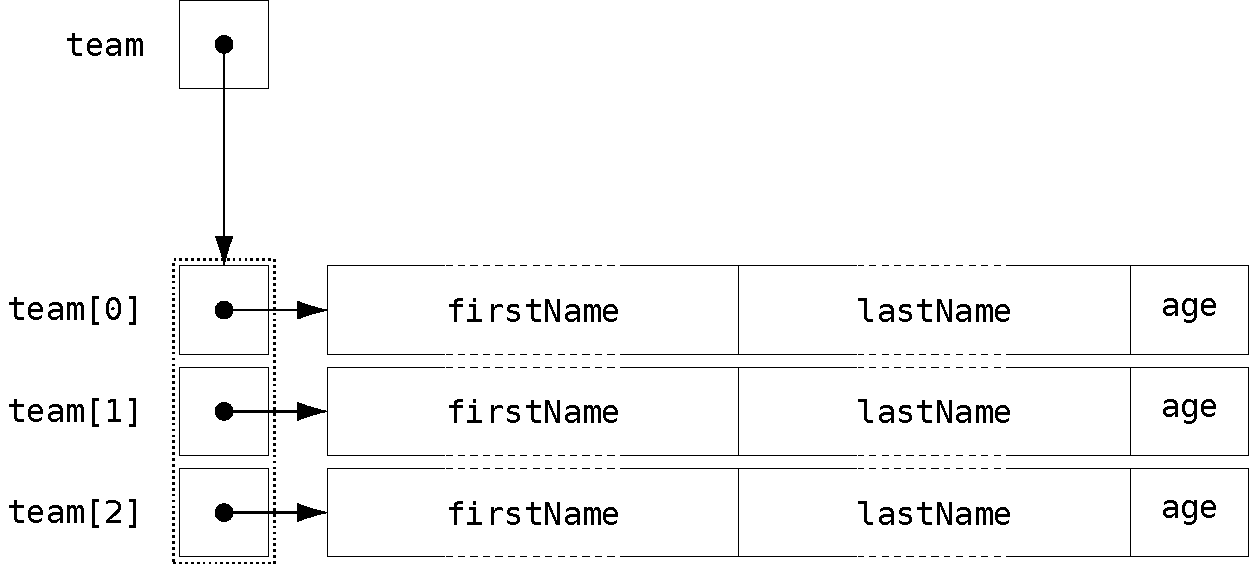
\includegraphics[scale=0.7]{images/sortPlayers.pdf}
    \caption{Darstellung des Pointers auf ein Array von Pointern auf
    \mintinline{c}{Player}-Objekte}
    \label{fig:sortPlayer}
\end{figure}

Vergegenwertigen Sie sich an dieser Stelle auch den Inhalt der Pointer der
Vergleichsfunktion:

\noindent\mintinline{c}{comparePlayerByLastName(const void *pa, const void *pb)}

Die beiden Pointer \mintinline{c}{pa} und \mintinline{c}{pb} zeigen beide
jeweils auf ein Array-Element des Arrays \mintinline{c}{team} und enthalten
dementsprechend selbst wieder einen Pointer auf ein
\mintinline{c}{Player}-Objekt.
